\chapter{Implementation: the SoundSuggest application}\label{chapter:implementation}

The application that was built for this thesis is called \emph{SoundSuggest}. It is a chrome extension that uses the D3 JavaScript library and the Last.fm API to inject the explanation system into the recommendations page of Last.fm\footnote{\url{http://www.last.fm/home/recs}}. In this chapter we will discuss the technologies we have used to create the application, the software design of the application and some specifics about the implementation of the application.


\section{Technologies}\label{chapter:implementation:section:technologies}

\subsection{Chrome extensions}\label{chapter:implementation:section:technologies:subsection:chrome}

Chrome Extensions are applications written in \emph{HTML}\index{HTML}, \emph{JavaScript}\index{JavaScript} and \emph{CSS}\index{CSS}\index{Cascading style sheet|see{CSS}}, that enhance to functionality of the Google Chrome web browser\cite{google:2012:extensions}.

There are different types of extensions. Browser actions are applications that can be launched regardless of the web page you are at. They appear as a button with a specified logo in the toolbar of the Chrome browser. By clicking the browser action you can specify to open up a tooltip or a popup\cite{google:2012:browseraction}. Page action extensions are meant to be shown when browsing specific web pages. They appear as an icon in the address bar. Page actions use content scripts to inject code into the web page\cite{google:2012:overview}.

The file \emph{manifest.JSON} is one of the key areas of a chrome extension. It specifies the name and the version of your application as well as other important settings such as the type of the extension, scripts and security policies\cite{google:2012:manifest}.

Many extensions use a two-layered structure in which you have a background page and UI pages or content scripts\cite{google:2012:overview}. In the usual case the views are stateless and background pages are not. When the view needs some state, it requests the state from the background page. When the background page notices a state change, the background page tells the views to update\cite{google:2012:background}. Background pages can either be persistent or not. In the last case we are talking about so called event pages; they are opened and closed as needed\cite{google:2012:overview}.

There are various ways to use UI pages: you can open an HTML page in a popup, another tab or options page. The HTML pages inside an extension have complete access to each other's DOMs, and they can invoke functions on each other\cite{google:2012:overview}.

Content scripts are JavaScript scripts that are used to interact with a webpage opened in a browser tab. An important remark is that you should consider a content script part of the webpage it is injected into, rather than its parent extension. It can modify the DOM of the webpage but not the DOM of its background page. However it can ask its background page for data through listeners in the background page's script\cite{google:2012:overview}.



\subsection{The Last.fm API}\label{chapter:implementation:section:technologies:subsection:lastfm}

The \emph{Last.fm API}\footnote{\url{http://www.last.fm/api}} offers great functionality such as the recommender system, Last.fm scrobbling and accessing and modifying your Last.fm profile information, aside from providing a large amount of data. To use the API, libraries have been developed for several technologies, such as \emph{JavaScript}\index{JavaScript}, \emph{PHP}, \emph{Python} and \emph{Actionscript} among others\cite{lastfm:2012:home}.

To build an application using the Last.fm API, you have to create an API account first at \url{http://www.last.fm/api/account/create}. Once you have been registered, you will receive an API key and an API secret.

For testing purposes it will also be handy to have a Last.fm account of your own. So if you haven't got one already sign up at their website. You might also want to one or more of their \emph{Scrobbler}\index{Scrobbler} applications. This will collect data from your music players to generate profile information that will be used to generate recommendations\cite{lastfm:2013:scrobbling}.

There are already several interesting applications that make use of the Last.fm API. Even more interesting perhaps is that some developers distribute free JavaScript libraries that act like a facade on the Last.fm API. The JavaScript library we will be using here, can be found on \emph{GitHub}\footnote{\url{https://github.com/fxb/javascript-last.fm-api}} and is written by \emph{Felix Bruns}.


\subsection{D3.js JavaScript Library}\label{chapter:implementation:section:technologies:subsection:d3js}

Visualizations for web applications can be built using \emph{scalable vector graphics}\index{scalable vector graphics} \emph{(SVG)\index{SVG|see{scalable vector graphics}}}. SVG is an XML-based language to describe two-dimensional graphics\cite{w3c:2011:svg}. It is supported by most of the latest versions of most popular browsers, including \emph{Chrome}, \emph{Firefox}, \emph{Internet Explorer 9}, \emph{Opera} and \emph{Safari}\cite{microsoft:2012:svg, w3c:2010:svg}.

\emph{D3.js}\index{D3.js} is a JavaScript library that uses the W3C standards \emph{HTML}, \emph{SVG} and \emph{CSS} to build data-driven documents\index{data-driven documents|see{D3.js}}\cite{bostock:2012:d3js}. There are various tutorials explaining the basics on how to use this library.

In short, to get started the library should be included in your web page. Next, using the D3 selectors, elements can be added and removed easily from the web page. The library also offers a number of built-in algorithms, as well as a series of example visualizations that can be customized as desired.


\subsection{Additional libraries}\label{chapter:implementation:section:technologies:subsection:libs}

In addition to the Last.fm API JavaScript library and D3.js, four other JavaScript libraries were used, namely:

\begin{itemize}
	\item \textbf{jQuery}\footnote{\url{http://jquery.com/}}: "jQuery is a fast, small, and feature-rich JavaScript library. It makes things like HTML document traversal and manipulation, event handling, animation, and Ajax much simpler with an easy-to-use API that works across a multitude of browsers"\cite{jquery:2013}.
	\item \textbf{jQuery UI}\footnote{\url{}}: "jQuery UI is a curated set of user interface interactions, effects, widgets, and themes built on top of the jQuery JavaScript Library"\cite{jqueryui:2013}.
	\item \textbf{Purl.js}\footnote{\url{https://github.com/allmarkedup/jQuery-URL-Parser}}: a library built on the jQuery library to retrieve GET parameters from the web page's URL.
	\item \textbf{Spinner.js}\footnote{\url{http://fgnass.github.io/spin.js/}}: a library that creates a spinner element with given parameters for customization.
\end{itemize}


\section{Software design and application architecture}\label{chapter:implementation:section:design}

% Life lines :
%		ACTOR
%		(UI)
%		content script
%		background script
%		Local storage
%		Last.fm API


\begin{figure}%
	\begin{center}
		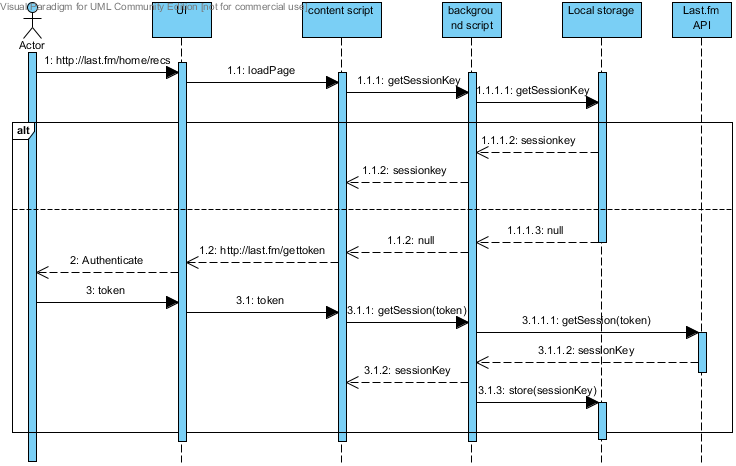
\includegraphics[width=\columnwidth]{img/seq_part1}%
	\end{center}
	\caption{Sequence diagram: opening the Last.fm recommendations page part 1: retrieving a session key.}%
	\label{fig:sequence:part1}%
\end{figure}

\begin{figure}%
	\begin{center}
		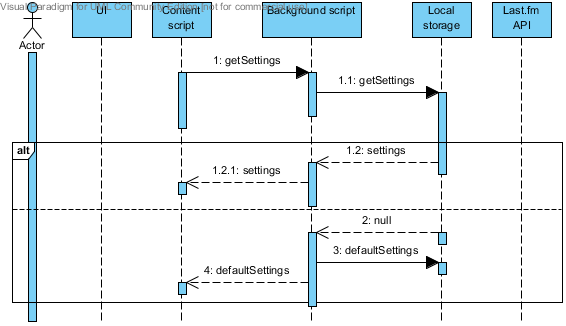
\includegraphics[width=\columnwidth]{img/seq_part2}%
	\end{center}
	\caption{Sequence diagram: opening the Last.fm recommendations page part 2: retrieving stored settings.}%
	\label{fig:sequence:part2}%
\end{figure}

\begin{figure}%
	\begin{center}
		\includegraphics[width=\columnwidth]{img/seq_settings}%
	\end{center}
	\caption{Sequence diagram: changing settings.}%
	\label{fig:sequence:settings}%
\end{figure}



\section{Implementation}\label{chapter:implementation:section:implementation}








